\chapter{Portfolio Optimization}\label{portfolio-optimization}

Portfolio optimization models look for the optimal way to make investments. Usually investors expect 
either a maximum return for a given level of risk or a given return for a minimum risk so these models
are typically based on two criteria: maximization of the expected return and/or minimization of the risk.

While the concept of return is straightforward there is a variety of measures of risk. 
The most popular one has been variance in return and we will first look at it very closely before 
introducing some alternatives.

Some notations that will be used later are

\begin{itemize}
\tightlist
\item
  expected return: \[ \mathbb{E}(R_{p}) = \sum _{i}w_{i} \mathbb{E}(R_{i}) \] where
  \(R_{p}\) is the return on the portfolio, \(R_{i}\) is the return on
  asset \(i\) and \(w_{i}\) is the weighting of component asset \(i\)
  (that is, the proportion of asset \(i\) in the portfolio) and
  \(\sum_{i}w_i = 1\) and \(0 \le w_i \le 1\);
\item
  portfolio return variance:
  \[ \sigma _{p}^{2} = \sum _{i}w_{i}^{2}\sigma _{i}^{2} + \sum _{i}\sum _{j\neq i}w_{i}w_{j}\sigma _{i}\sigma _{j}\rho _{ij} \]
  where \(\sigma\) is the (sample) standard deviation of the periodic
  returns on an asset, and \(\rho _{ij}\) is the correlation coefficient
  between the returns on assets \(i\) and \(j\). In a more compact way
  it can be expressed as:
  \[ \sigma _{p}^{2}=\sum _{i}\sum _{j}w_{i}w_{j}\sigma _{ij} \] where
  \(\sigma _{ij}=\sigma _{i}\sigma _{j}\rho _{ij}\) is the (sample)
  covariance of the periodic returns on the two assets, or alternatively
  denoted as \(\Sigma\).
  In matrix notation:
  \[\sigma_p^2 = \mathbf{w^T}\Sigma\mathbf{w} \]
  where $\mathbf{w} = (w_1,w_2,\ldots,w_N)$ is the vector of weights. 
  For a very brief introduction to matrices see Appendix~\ref{app:matrices};
\item
  portfolio return volatility (standard deviation):
  \[ \sigma _{p}= \sqrt{\sigma _{p}^{2}}\]
\end{itemize}

\section{The Markowitz Mean/Variance Portfolio Model}
\label{the-markowitz-meanvariance-portfolio-model}

This model, first introduced by Markowitz, assumes that an investor has
two considerations when constructing an investment portfolio: expected
return and variance in return (i.e. measure of risk or of the
variability in realized return around the expected return). Hence the
Markowitz model requires two major kinds of information:

\begin{itemize}
\tightlist
\item
  the estimated expected return for each candidate investment;
\item
  the covariance matrix of returns, which characterizes not only the 
  individual variability of the return on each investment, 
  but also how each investment's return tends to move with the other (correlation).
\end{itemize}

In the example proposed in this Chapter we are going to use real data
of five companies:  AAPL, AMZN, FB, GOOG, NFLX.
Data, shown in Figure~\ref{fig:stocks}, is made of the historical 
series of the closing prices in the last 5 years which are saved in 
\href{https://drive.google.com/file/d/1srCzNlKVY_LHRpkaKoUynnmI0KImfT6Y/view?usp=sharing}{portfolio\_data.csv}.

\begin{tcolorbox}[breakable, size=fbox, boxrule=1pt, pad at break*=1mm,colback=cellbackground, colframe=cellborder]
\begin{Verbatim}[commandchars=\\\{\}]
\PY{k+kn}{import} \PY{n+nn}{pandas} \PY{k}{as} \PY{n+nn}{pd}
		
\PY{n}{df} \PY{o}{=} \PY{n}{pd}\PY{o}{.}\PY{n}{read\PYZus{}csv}\PY{p}{(}\PY{l+s+s2}{\PYZdq{}}\PY{l+s+s2}{portfolio\PYZus{}data.csv}\PY{l+s+s2}{\PYZdq{}}\PY{p}{,} \PY{n}{index\PYZus{}col}\PY{o}{=}\PY{l+s+s2}{\PYZdq{}}\PY{l+s+s2}{date}\PY{l+s+s2}{\PYZdq{}}\PY{p}{)}
\PY{n+nb}{print} \PY{p}{(}\PY{n}{df}\PY{o}{.}\PY{n}{head}\PY{p}{(}\PY{p}{)}\PY{p}{)}

                 AAPL     AMZN     FB    GOOG       NFLX
date
2014-03-27  71.865678  338.470  60.97  558.46  52.025714
2014-03-28  71.785450  338.290  60.01  559.99  51.267143
2014-03-31  71.769404  336.365  60.24  556.97  50.290000
2014-04-01  72.425937  342.990  62.62  567.16  52.098571
2014-04-02  72.546280  341.960  62.72  567.00  51.840000
\end{Verbatim}
\end{tcolorbox}

With \texttt{pandas} the main characteristics of these time series can
be easily computed (e.g. daily returns, covariance matrix,\ldots):

\begin{tcolorbox}[breakable, size=fbox, boxrule=1pt, pad at break*=1mm,colback=cellbackground, colframe=cellborder]
\begin{Verbatim}[commandchars=\\\{\}]
\PY{n}{daily\PYZus{}returns} \PY{o}{=} \PY{n}{df}\PY{o}{.}\PY{n}{pct\PYZus{}change}\PY{p}{(}\PY{p}{)}
\PY{n}{returns} \PY{o}{=} \PY{n}{daily\PYZus{}returns}\PY{o}{.}\PY{n}{mean}\PY{p}{(}\PY{p}{)}\PY{o}{*}\PY{l+m+mi}{252}
\PY{n+nb}{print} \PY{p}{(}\PY{n}{returns}\PY{p}{)}

AAPL    0.239188
AMZN    0.415127
FB      0.263797
GOOG    0.172818
NFLX    0.528046
dtype: float64
\end{Verbatim}
\end{tcolorbox}

\begin{tcolorbox}[breakable, size=fbox, boxrule=1pt, pad at break*=1mm,colback=cellbackground, colframe=cellborder]
\begin{Verbatim}[commandchars=\\\{\}]
\PY{n}{covariance} \PY{o}{=} \PY{n}{daily\PYZus{}returns}\PY{o}{.}\PY{n}{cov}\PY{p}{(}\PY{p}{)}\PY{o}{*}\PY{l+m+mi}{252}
\PY{n+nb}{print} \PY{p}{(}\PY{n}{covariance}\PY{p}{)}

          AAPL      AMZN        FB      GOOG      NFLX
AAPL  0.051902  0.025037  0.025737  0.022454  0.027760
AMZN  0.025037  0.085839  0.041025  0.039501  0.048412
FB    0.025737  0.041025  0.069550  0.036127  0.044528
GOOG  0.022454  0.039501  0.036127  0.051797  0.040390
NFLX  0.027760  0.048412  0.044528  0.040390  0.178298
\end{Verbatim}
\end{tcolorbox}

\begin{figure}[htb]
\centering
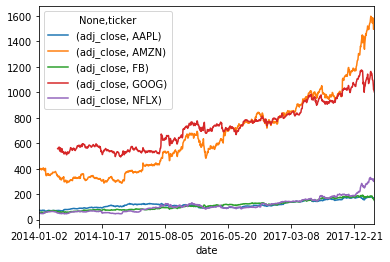
\includegraphics[width=0.7\textwidth]{figures/portfolio_sample}
\caption{Historical series of the closing price of five companies. To compare them, prices, have been normalized to the 
first value in each series}
\label{fig:stocks}
\end{figure}
    
In order to "simulate" a portfolio it is enough to throw five random weights 
with the constraint that they had to sum up to 1. 
In Figure~\ref{fig:mc_portfolio} a large number of simulated portfolios are shown in the return vs volatility plane. 
In this case no attempt of any optimization whatsoever has been made.

\begin{figure}[hbt]
\centering
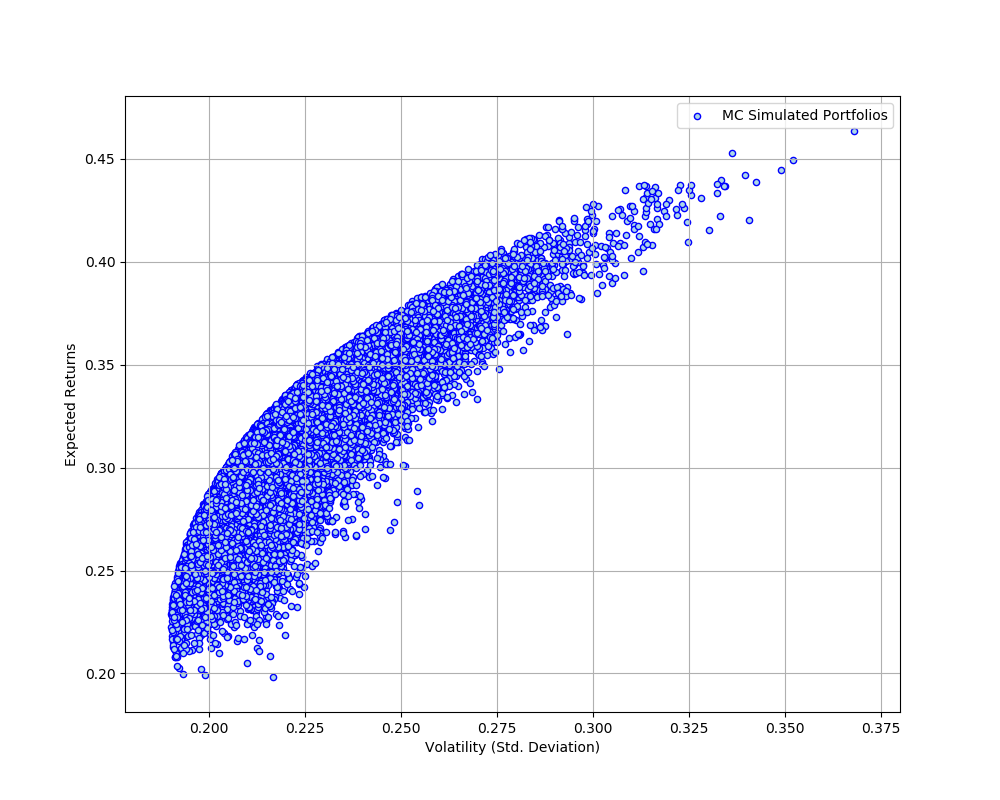
\includegraphics[width=0.8\textwidth]{figures/return_variance}
\caption{Distribution in the expected return/volatility plane of a large number of simulated portfolios.}
\label{fig:mc_portfolio}
\end{figure}

Investors may use short sales in their portfolios (a portfolio is short in those stocks with negative portfolio weights). 
Although short selling extends the set of possible portfolios we are not going to consider them here.

\section{Optimisation}\label{optimization}

Markowitz model states that the weights of a portfolio should be chosen 
such that its volatility (or its variance) is minimised. 
So the application of this model reduces to
an optimisation problem: given the covariance matrix of the portfolio
$\Sigma$, estimated from their historical series, we need to find

\[\underset{\mathbf{w}}{\min}\{\sigma_p^2\} = \underset{\mathbf{w}}{\min}\{\mathbf{w^T}\Sigma\mathbf{w}\}\]
with the constraints \(\sum_{i}w_i = 1\) and \(0 \le w_i \le 1\).

In \texttt{python} we already know how to solve a minimisation problem
(see bootstrapping in Chapter~\ref{swaps-and-bootstrapping---practical-lesson-5}) 
so it is enough to repeat the same steps:

\begin{itemize}
\tightlist
\item
  define an objective function (in this case the portfolio variance);
\item
  define a set of constraints ($\sum w_i = 1$);
\item
  set an initial guess for the weights;
\item
  pass everything to \texttt{scipy.optimize.minimize}.
\end{itemize}

\begin{tcolorbox}[breakable, size=fbox, boxrule=1pt, pad at break*=1mm,colback=cellbackground, colframe=cellborder]
\begin{Verbatim}[commandchars=\\\{\}]
\PY{k+kn}{import} \PY{n+nn}{numpy} \PY{k}{as} \PY{n+nn}{np}
\PY{k+kn}{from} \PY{n+nn}{scipy}\PY{n+nn}{.}\PY{n+nn}{optimize} \PY{k}{import} \PY{n}{minimize}
		
\PY{k}{def} \PY{n+nf}{sum\PYZus{}weights}\PY{p}{(}\PY{n}{w}\PY{p}{)}\PY{p}{:} 
    \PY{k}{return} \PY{n}{np}\PY{o}{.}\PY{n}{sum}\PY{p}{(}\PY{n}{w}\PY{p}{)} \PY{o}{\PYZhy{}} \PY{l+m+mi}{1}
		
\PY{k}{def} \PY{n+nf}{markowitz}\PY{p}{(}\PY{n}{w}\PY{p}{,} \PY{n}{cov}\PY{p}{)}\PY{p}{:}
    \PY{k}{return} \PY{n}{w}\PY{o}{.}\PY{n}{T}\PY{o}{.}\PY{n}{dot}\PY{p}{(}\PY{n}{cov}\PY{o}{.}\PY{n}{dot}\PY{p}{(}\PY{n}{w}\PY{p}{)}\PY{p}{)}
		
\PY{n}{num\PYZus{}assets} \PY{o}{=} \PY{l+m+mi}{5}
\PY{n}{constraints} \PY{o}{=} \PY{p}{(}\PY{p}{\PYZob{}}\PY{l+s+s1}{\PYZsq{}}\PY{l+s+s1}{type}\PY{l+s+s1}{\PYZsq{}}\PY{p}{:} \PY{l+s+s1}{\PYZsq{}}\PY{l+s+s1}{eq}\PY{l+s+s1}{\PYZsq{}}\PY{p}{,} \PY{l+s+s1}{\PYZsq{}}\PY{l+s+s1}{fun}\PY{l+s+s1}{\PYZsq{}}\PY{p}{:} \PY{n}{sum\PYZus{}weights}\PY{p}{\PYZcb{}}\PY{p}{,}\PY{p}{)} 
\PY{n}{bounds} \PY{o}{=} \PY{n+nb}{tuple}\PY{p}{(}\PY{p}{(}\PY{l+m+mi}{0}\PY{p}{,} \PY{l+m+mi}{1}\PY{p}{)} \PY{k}{for} \PY{n}{asset} \PY{o+ow}{in} \PY{n+nb}{range}\PY{p}{(}\PY{n}{num\PYZus{}assets}\PY{p}{)}\PY{p}{)}
\PY{n}{weights} \PY{o}{=} \PY{p}{[}\PY{l+m+mf}{1.}\PY{o}{/}\PY{n}{num\PYZus{}assets} \PY{k}{for} \PY{n}{\PYZus{}} \PY{o+ow}{in} \PY{n+nb}{range}\PY{p}{(}\PY{n}{num\PYZus{}assets}\PY{p}{)}\PY{p}{]}
		
\PY{n}{opts} \PY{o}{=} \PY{n}{minimize}\PY{p}{(}\PY{n}{markowitz}\PY{p}{,} \PY{n}{weights}\PY{p}{,} \PY{n}{args}\PY{o}{=}\PY{p}{(}\PY{n}{covariance}\PY{p}{,}\PY{p}{)}\PY{p}{,}
                \PY{n}{bounds}\PY{o}{=}\PY{n}{bounds}\PY{p}{,} \PY{n}{constraints}\PY{o}{=}\PY{n}{constraints}\PY{p}{)}
\PY{n+nb}{print} \PY{p}{(}\PY{n}{opts}\PY{p}{)}

    fun: 0.03607029963784209
    jac: array([0.0723022 , 0.07233166, 0.0718961 , 0.07199311, 0.07223676])
message: 'Optimization terminated successfully.'
   nfev: 63
    nit: 9
   njev: 9
 status: 0
success: True
      x: array([0.44544146, 0.06252825, 0.12333117, 0.3662157 , 0.00248342])

\PY{n+nb}{print} \PY{p}{(}\PY{l+s+s2}{\PYZdq{}}\PY{l+s+s2}{Expected portfolio return: }\PY{l+s+si}{\PYZob{}:.3f\PYZcb{}}\PY{l+s+s2}{\PYZdq{}}\PY{o}{.}\PY{n}{format}\PY{p}{(}\PY{n}{np}\PY{o}{.}\PY{n}{dot}\PY{p}{(}\PY{n}{opts}\PY{o}{.}\PY{n}{x}\PY{p}{,} \PY{n}{returns}\PY{p}{)}\PY{p}{)}\PY{p}{)}

Expected portfolio return: 0.230
\end{Verbatim}
\end{tcolorbox}

The solution recommends to devote about 44\% of the portfolio to AAPL,
about 6\% to AMZN, 12\% to FB and so on\ldots 
The expected return is
about 23\%, with a variance of about 0.036 or, equivalently, a standard deviation of 0.19.

In this example we based the model simply on straightforward statistical
data derived from daily returns. However it could be possible, rather
than estimate the expected returns form historical data,
to base this estimate on information about
expected future performance of the asset.

\section{Efficient Frontier}\label{efficient-frontier}
There is no precise way for an investor to determine the “correct” trade off between risk and return. If she wants a higher expected return, she generally has to “pay for it” with higher risk. Thus, one is frequently interested in looking at the relative distribution of the two.

In finance terminology, we would like to trace out the \emph{efficient frontier} of return and risk. This is doable solving for the minimum variance portfolio over a range of values for the expected return (e.g. ranging from 0.20 to 0.45).

This time beside the constraint on the sum of weights, we have to add the one that forces the resulting return to be equal to the chosen target.

The following example produce the efficient frontier plot shown in Fig.~\ref{fig:efficient_frontier}.

\begin{tcolorbox}[breakable, size=fbox, boxrule=1pt, pad at break*=1mm,colback=cellbackground, colframe=cellborder]
\begin{Verbatim}[commandchars=\\\{\}]
\PY{k}{def} \PY{n+nf}{efficient\PYZus{}frontier}\PY{p}{(}\PY{n}{w}\PY{p}{,} \PY{n}{asset\PYZus{}returns}\PY{p}{,} \PY{n}{target\PYZus{}return}\PY{p}{)}\PY{p}{:} 
    \PY{n}{portfolio\PYZus{}return} \PY{o}{=} \PY{n}{asset\PYZus{}returns}\PY{o}{.}\PY{n}{dot}\PY{p}{(}\PY{n}{w}\PY{p}{)} 
    \PY{k}{return} \PY{p}{(}\PY{n}{portfolio\PYZus{}return} \PY{o}{\PYZhy{}} \PY{n}{target\PYZus{}return}\PY{p}{)}
		
\PY{n}{results} \PY{o}{=} \PY{p}{[}\PY{p}{]}
\PY{n}{bounds} \PY{o}{=} \PY{n+nb}{tuple}\PY{p}{(}\PY{p}{(}\PY{l+m+mi}{0}\PY{p}{,} \PY{l+m+mi}{1}\PY{p}{)} \PY{k}{for} \PY{n}{asset} \PY{o+ow}{in} \PY{n+nb}{range}\PY{p}{(}\PY{n}{num\PYZus{}assets}\PY{p}{)}\PY{p}{)}
		
\PY{k}{for} \PY{n}{eff} \PY{o+ow}{in} \PY{n}{np}\PY{o}{.}\PY{n}{arange}\PY{p}{(}\PY{l+m+mf}{0.20}\PY{p}{,} \PY{l+m+mf}{0.45}\PY{p}{,} \PY{l+m+mf}{0.005}\PY{p}{)}\PY{p}{:}
    \PY{n}{constraints} \PY{o}{=} \PY{p}{(}\PY{p}{\PYZob{}}\PY{l+s+s1}{\PYZsq{}}\PY{l+s+s1}{type}\PY{l+s+s1}{\PYZsq{}}\PY{p}{:} \PY{l+s+s1}{\PYZsq{}}\PY{l+s+s1}{eq}\PY{l+s+s1}{\PYZsq{}}\PY{p}{,} \PY{l+s+s1}{\PYZsq{}}\PY{l+s+s1}{fun}\PY{l+s+s1}{\PYZsq{}}\PY{p}{:} \PY{n}{efficient\PYZus{}frontier}\PY{p}{,} 
                    \PY{l+s+s1}{\PYZsq{}}\PY{l+s+s1}{args}\PY{l+s+s1}{\PYZsq{}}\PY{p}{:}\PY{p}{(}\PY{n}{returns}\PY{p}{,} \PY{n}{eff}\PY{p}{,}\PY{p}{)}\PY{p}{\PYZcb{}}\PY{p}{,}
                   \PY{p}{\PYZob{}}\PY{l+s+s1}{\PYZsq{}}\PY{l+s+s1}{type}\PY{l+s+s1}{\PYZsq{}}\PY{p}{:} \PY{l+s+s1}{\PYZsq{}}\PY{l+s+s1}{eq}\PY{l+s+s1}{\PYZsq{}}\PY{p}{,} \PY{l+s+s1}{\PYZsq{}}\PY{l+s+s1}{fun}\PY{l+s+s1}{\PYZsq{}}\PY{p}{:} \PY{n}{sum\PYZus{}weights}\PY{p}{\PYZcb{}}\PY{p}{)}
    \PY{n}{weights} \PY{o}{=} \PY{p}{[}\PY{l+m+mf}{1.}\PY{o}{/}\PY{n}{num\PYZus{}assets} \PY{k}{for} \PY{n}{\PYZus{}} \PY{o+ow}{in} \PY{n+nb}{range}\PY{p}{(}\PY{n}{num\PYZus{}assets}\PY{p}{)}\PY{p}{]}
    \PY{n}{opts} \PY{o}{=} \PY{n}{minimize}\PY{p}{(}\PY{n}{markowitz}\PY{p}{,} \PY{n}{weights}\PY{p}{,} \PY{n}{args}\PY{o}{=}\PY{p}{(}\PY{n}{covariance}\PY{p}{,}\PY{p}{)}\PY{p}{,}
                    \PY{n}{bounds}\PY{o}{=}\PY{n}{bounds}\PY{p}{,} \PY{n}{constraints}\PY{o}{=}\PY{n}{constraints}\PY{p}{)} 
		
    \PY{n}{results}\PY{o}{.}\PY{n}{append}\PY{p}{(}\PY{p}{(}\PY{n}{np}\PY{o}{.}\PY{n}{sqrt}\PY{p}{(}\PY{n}{opts}\PY{o}{.}\PY{n}{x}\PY{o}{.}\PY{n}{T}\PY{o}{.}\PY{n}{dot}\PY{p}{(}\PY{n}{covariance}\PY{o}{.}\PY{n}{dot}\PY{p}{(}\PY{n}{opts}\PY{o}{.}\PY{n}{x}\PY{p}{)}\PY{p}{)}\PY{p}{)}\PY{p}{,}
                    \PY{n}{np}\PY{o}{.}\PY{n}{sum}\PY{p}{(}\PY{n}{returns}\PY{o}{*}\PY{n}{opts}\PY{o}{.}\PY{n}{x}\PY{p}{)}\PY{p}{)}\PY{p}{)} 
\end{Verbatim}
\end{tcolorbox}

\begin{figure}[htb]
\centering
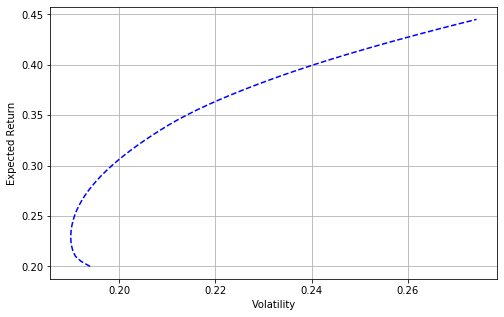
\includegraphics[width=0.7\textwidth]{figures/efficient_frontier.png}
\caption{Efficient frontier for our example portfolio obtained minimizing the the variance and requiring an expected return between 0.02 and 0.45.}
\label{fig:efficient_frontier}
\end{figure}

Efficient portfolios offer investors the highest possible expected return for a given level of risk. As investors add stocks to a portfolio, the efficient portfolio improves.
An investor seeking high expected returns and low volatility should invest only in efficient portfolios and will choose from the set of efficient portfolios based on her risk tolerance.
    
\subsection{Limits of the Markowitz Model}
 \label{limits-of-the-markowitz-model}
    
Despite the significant utility of the Markowitz theory, there are some major limitations in this model:
    
\begin{itemize}
  	\tightlist
   	\item
   	it is difficult to forecast asset returns with accuracy using
   	historical data, which tends to be a poor forecasting source. As
   	return estimations have a much larger impact on the asset allocations,
   	small changes in return assumptions can lead to inefficient
   	portfolios. Therefore, the model tends to lead to highly concentrated
   	portfolios (out-of sample weights) that do not offer as much
   	diversification benefits in practice as they seem to provide in
   	theory;
    	\item
    	the model assumes that asset correlations are linear. In reality,
    	asset correlations move dynamically, changing with the market cycles.
    	During the global financial crisis, asset correlations approached
    	almost 1, so if anything, diversification seemed to have insignificant
    	impacts on the portfolios;
    	\item
    	last but not the least, the model assumes normality in return
    	distributions. Therefore, it does not factor in extreme market moves
    	which tend to make returns distributions either skewed, fat tailed or
    	both. Without optimising the portfolio for asset that may actually
    	have skewed distributions or fat tailed, it could lead to a riskier
    	allocation that is intended.
    \end{itemize}
    
Extensions of the Markowitz model are the  \href{https://en.wikipedia.org/wiki/Post-modern_portfolio_theory}{Post Modern Theory} and the \href{https://en.wikipedia.org/wiki/Black\%E2\%80\%93Litterman_model}{Black-Litterman Model}.
    
\section{Portfolios with a Risk-Free Asset}
\label{portfolios-with-a-risk-free-asset}

When one of the investments available is risk free, then the efficient
frontier has a particularly simple form. The risk–return combinations of the risk-free investment and a risky portfolio lie on a straight line connecting the two investments: the capital allocation line (CAL). The slope of the CAL measures the trade off
between risk and return. A higher slope means that investors receive a
higher expected return in exchange for taking on more risk.

The capital allocation line aids investors in choosing how much to
invest in a risk-free asset and one or more risky assets.

The simplest example of such kind of portfolios is the one containing only two assets: a risk-free Treasury bill and a stock. Assume that the expected return of the Treasury bill is \(\mathbb{E}(R_f)=3\%\) and its risk is 0\%. Further, assume that the expected return of the stock is \(\mathbb{E}(R_r)=10\%\) and its standard deviation is \(\sigma_r=20\%\). The question that needs to be answered
for any individual investor is how much to invest in each of these
assets.

The expected return (\(\mathbb{E}(R_p)\)) of this portfolio is calculated as follows:

\[ \mathbb{E}(R_p) = \mathbb{E}(R_f)\cdot w_f + \mathbb{E}(R_r)\cdot (1- w_f) \]
where \(w_f\) is the relative allocation to the risk-free asset.

The calculation of risk for this portfolio is simple because the
standard deviation of the Treasury bill is 0\%. Thus it is calculated
as

\[ \sigma_p = (1-w_f)\cdot \sigma_r \]

In this very simple example, if an investor invested 100\% into
the risk-free asset (\(w_f=1\)), the expected return would be 3\% and
the risk of the portfolio would be 0\%. Likewise, investing 100\% into
the stock (\(w_f=0\)) would give an investor an expected return of 10\%
and a portfolio risk of 20\%. If the investor allocated 25\% to the
risk-free asset and 75\% to the risky asset, the portfolio expected
return and risk calculations would be

\[ \mathbb{E}(R_p) = (3\% \cdot 25\%) + (10\% \cdot 75\%) = 0.75\% + 7.5\% = 8.25\% \]

\[ \sigma_p = 75\% \cdot 20\% = 15\% \]

Applying the same reasoning to our example we can consider an additional
risk-free asset with an expected return of 10\% and repeat the
minimisation to determine the efficient frontier of the resulting
portfolio. Notice how the objective function is almost the same as before, 
while the target return constraint now includes the risk-free asset.

\begin{tcolorbox}[breakable, size=fbox, boxrule=1pt, pad at break*=1mm,colback=cellbackground, colframe=cellborder]
\begin{Verbatim}[commandchars=\\\{\}]
\PY{n}{num\PYZus{}assets} \PY{o}{=} \PY{l+m+mi}{6}
		
\PY{k}{def} \PY{n+nf}{markowitz\PYZus{}with\PYZus{}rf}\PY{p}{(}\PY{n}{w}\PY{p}{,} \PY{n}{cov}\PY{p}{)}\PY{p}{:}
    \PY{k}{return} \PY{n}{w}\PY{p}{[}\PY{p}{:}\PY{o}{\PYZhy{}}\PY{l+m+mi}{1}\PY{p}{]}\PY{o}{.}\PY{n}{T}\PY{o}{.}\PY{n}{dot}\PY{p}{(}\PY{n}{cov}\PY{o}{.}\PY{n}{dot}\PY{p}{(}\PY{n}{w}\PY{p}{[}\PY{p}{:}\PY{o}{\PYZhy{}}\PY{l+m+mi}{1}\PY{p}{]}\PY{p}{)}\PY{p}{)}
		
\PY{k}{def} \PY{n+nf}{efficient\PYZus{}frontier\PYZus{}with\PYZus{}rf}\PY{p}{(}\PY{n}{w}\PY{p}{,} \PY{n}{asset\PYZus{}returns}\PY{p}{,} \PY{n}{target\PYZus{}return}\PY{p}{,} \PY{n}{risk\PYZus{}free}\PY{p}{)}\PY{p}{:} 
    \PY{n}{portfolio\PYZus{}return} \PY{o}{=} \PY{n}{np}\PY{o}{.}\PY{n}{sum}\PY{p}{(}\PY{n}{asset\PYZus{}returns}\PY{o}{*}\PY{n}{w}\PY{p}{[}\PY{p}{:}\PY{o}{\PYZhy{}}\PY{l+m+mi}{1}\PY{p}{]}\PY{p}{)} \PY{o}{+} \PY{n}{risk\PYZus{}free}\PY{o}{*}\PY{n}{w}\PY{p}{[}\PY{l+m+mi}{5}\PY{p}{]} 
    \PY{k}{return} \PY{p}{(}\PY{n}{portfolio\PYZus{}return} \PY{o}{\PYZhy{}} \PY{n}{target\PYZus{}return}\PY{p}{)}
	
\PY{n}{rf\PYZus{}asset\PYZus{}return} \PY{o}{=} \PY{l+m+mf}{0.10}
\PY{n}{results\PYZus{}rf} \PY{o}{=} \PY{p}{[}\PY{p}{]}
\PY{n}{bounds} \PY{o}{=} \PY{n+nb}{tuple}\PY{p}{(}\PY{p}{(}\PY{l+m+mi}{0}\PY{p}{,} \PY{l+m+mi}{1}\PY{p}{)} \PY{k}{for} \PY{n}{asset} \PY{o+ow}{in} \PY{n+nb}{range}\PY{p}{(}\PY{n}{num\PYZus{}assets}\PY{p}{)}\PY{p}{)}
\PY{k}{for} \PY{n}{eff} \PY{o+ow}{in} \PY{n}{np}\PY{o}{.}\PY{n}{arange}\PY{p}{(}\PY{l+m+mf}{0.10}\PY{p}{,} \PY{l+m+mf}{0.45}\PY{p}{,} \PY{l+m+mf}{0.01}\PY{p}{)}\PY{p}{:}
    \PY{n}{constraints} \PY{o}{=} \PY{p}{(}\PY{p}{\PYZob{}}\PY{l+s+s1}{\PYZsq{}}\PY{l+s+s1}{type}\PY{l+s+s1}{\PYZsq{}}\PY{p}{:} \PY{l+s+s1}{\PYZsq{}}\PY{l+s+s1}{eq}\PY{l+s+s1}{\PYZsq{}}\PY{p}{,} \PY{l+s+s1}{\PYZsq{}}\PY{l+s+s1}{fun}\PY{l+s+s1}{\PYZsq{}}\PY{p}{:} \PY{n}{efficient\PYZus{}frontier\PYZus{}with\PYZus{}rf}\PY{p}{,} 
                     \PY{l+s+s2}{\PYZdq{}}\PY{l+s+s2}{args}\PY{l+s+s2}{\PYZdq{}}\PY{p}{:}\PY{p}{(}\PY{n}{returns}\PY{p}{,} \PY{n}{eff}\PY{p}{,} \PY{n}{rf\PYZus{}asset\PYZus{}return}\PY{p}{)}\PY{p}{\PYZcb{}}\PY{p}{,}
                    \PY{p}{\PYZob{}}\PY{l+s+s1}{\PYZsq{}}\PY{l+s+s1}{type}\PY{l+s+s1}{\PYZsq{}}\PY{p}{:} \PY{l+s+s1}{\PYZsq{}}\PY{l+s+s1}{eq}\PY{l+s+s1}{\PYZsq{}}\PY{p}{,} \PY{l+s+s1}{\PYZsq{}}\PY{l+s+s1}{fun}\PY{l+s+s1}{\PYZsq{}}\PY{p}{:} \PY{n}{sum\PYZus{}weights}\PY{p}{\PYZcb{}}\PY{p}{)}
    \PY{n}{weights} \PY{o}{=} \PY{p}{[}\PY{l+m+mf}{1.}\PY{o}{/}\PY{n}{num\PYZus{}assets} \PY{k}{for} \PY{n}{\PYZus{}} \PY{o+ow}{in} \PY{n+nb}{range}\PY{p}{(}\PY{n}{num\PYZus{}assets}\PY{p}{)}\PY{p}{]}
    \PY{n}{opts} \PY{o}{=} \PY{n}{minimize}\PY{p}{(}\PY{n}{markowitz\PYZus{}with\PYZus{}rf}\PY{p}{,} \PY{n}{weights}\PY{p}{,} \PY{n}{args}\PY{o}{=}\PY{p}{(}\PY{n}{covariance}\PY{p}{)}\PY{p}{,}
                    \PY{n}{bounds}\PY{o}{=}\PY{n}{bounds}\PY{p}{,} \PY{n}{constraints}\PY{o}{=}\PY{n}{constraints}\PY{p}{)}
    \PY{n}{results\PYZus{}rf}\PY{o}{.}\PY{n}{append}\PY{p}{(}\PY{p}{(}\PY{n}{np}\PY{o}{.}\PY{n}{sqrt}\PY{p}{(}\PY{n}{opts}\PY{o}{.}\PY{n}{x}\PY{p}{[}\PY{p}{:}\PY{o}{\PYZhy{}}\PY{l+m+mi}{1}\PY{p}{]}\PY{o}{.}\PY{n}{T}\PY{o}{.}\PY{n}{dot}\PY{p}{(}\PY{n}{covariance}\PY{o}{.}\PY{n}{dot}\PY{p}{(}\PY{n}{opts}\PY{o}{.}\PY{n}{x}\PY{p}{[}\PY{p}{:}\PY{o}{\PYZhy{}}\PY{l+m+mi}{1}\PY{p}{]}\PY{p}{)}\PY{p}{)}\PY{p}{)}\PY{p}{,} 
                       \PY{n}{np}\PY{o}{.}\PY{n}{sum}\PY{p}{(}\PY{n}{returns}\PY{o}{*}\PY{n}{opts}\PY{o}{.}\PY{n}{x}\PY{p}{[}\PY{p}{:}\PY{o}{\PYZhy{}}\PY{l+m+mi}{1}\PY{p}{]}\PY{p}{)}\PY{o}{+}\PY{n}{opts}\PY{o}{.}\PY{n}{x}\PY{p}{[}\PY{l+m+mi}{5}\PY{p}{]}\PY{o}{*}\PY{n}{rf\PYZus{}asset\PYZus{}return}\PY{p}{)}\PY{p}{)}
\end{Verbatim}
\end{tcolorbox}

\begin{figure}[htb]
\centering
    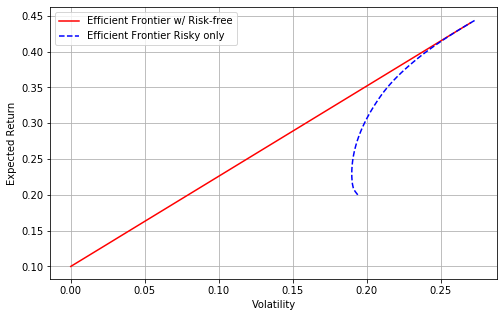
\includegraphics[width=0.7\textwidth]{figures/cal.png}
    \caption{Comparison of efficient frontier with a risk-free asset (red) and with risky asset only (blue).}
    \label{fig:cal}
\end{figure}
    
As it is clear from Fig.~\ref{fig:cal} the efficient frontier has become a
straight line, tangent to the frontier of the risky assets only. When
the target is 10\% the entire investment is allocated to the risk-free
asset, as the target increases the fraction of the risky assets grows
proportionally to the volatility. 

It is important to notice that in general the relative proportions
devoted to risky investments do not change. Only the allocation between
the risk-free asset and the risky assets change.

\subsection{The Sharpe Ratio}
\label{the-sharpe-ratio}
The goal of an investor who is seeking to earn the highest possible expected return for any 
level of volatility is to find the portfolio that generates the steepest possible line
when combined with the risk-free investment. The slope of the line is called the \emph{Sharpe ratio} of the portfolio.

For some portfolio of risky assets let

\begin{itemize}
\tightlist
\item
  \(R_r\) its expected return;
\item
  \(\sigma_r\) its standard deviation in return;
\item
  \(r_f\) the return of a risk-free asset.
\end{itemize}

A plausible single measure (as opposed to the two measures, risk and
return) of attractiveness of portfolio is the Sharpe ratio:

\[ \cfrac{R_r - r_f}{\sigma_r} \]

In words, it measures how much additional return we achieved for the
additional risk we took on, relative to putting all our money in the
risk-free asset. The portfolio that maximizes this ratio has some interesting properties. Suppose

\begin{itemize}
\tightlist
\item
  \(R_\textrm{target}\) our desired target return;
\item
  \(w_r\) the fraction of our wealth we place in the portfolio (the
  rest placed in the risk-free asset).
\end{itemize}

To meet our return target, we must have:

\[ (1 - w_r) * r_f + w_r * R_r =R_\textrm{target} \]

The standard deviation of our total investment is:
\(w_r\cdot \sigma_r\). Solving for \(w_r\) in the equation above, we
get:

\[ w_r = \cfrac{R_\textrm{target} - r_f}{R_r - r_f} \]

Thus, the standard deviation of the portfolio is:

\[ w_r\cdot \sigma_r = \left(\cfrac{R_\textrm{target} - r_f}{R_r - r_f}\right)\cdot \sigma_r \]

Minimising the portfolio standard deviation means:

\[ \textrm{min}\left[\cfrac{R_\textrm{target} - r_f}{R_r - r_f}\cdot \sigma_r\right]\implies\textrm{max}\left[\cfrac{R_r - r_f}{\sigma_r}\right] \]

So, regardless of our risk/return preference, the money we invest in
risky assets should be invested in the portfolio that maximises
the Sharpe ratio, because it will be also the portfolio that minimize 
the risk (i.e. standard deviation) at the same time.

Let's see the application of the Sharpe ratio on our sample.

\begin{tcolorbox}[breakable, size=fbox, boxrule=1pt, pad at break*=1mm,colback=cellbackground, colframe=cellborder]
\begin{Verbatim}[commandchars=\\\{\}]
\PY{n}{num\PYZus{}assets} \PY{o}{=} \PY{l+m+mi}{5}
\PY{n}{rf\PYZus{}asset\PYZus{}return} \PY{o}{=} \PY{l+m+mf}{0.10}
		
\PY{k}{def} \PY{n+nf}{negativeSharpeRatio}\PY{p}{(}\PY{n}{w}\PY{p}{,} \PY{n}{asset\PYZus{}returns}\PY{p}{,} \PY{n}{rf\PYZus{}asset\PYZus{}return}\PY{p}{,} \PY{n}{cov}\PY{p}{)}\PY{p}{:} 
    \PY{n}{p\PYZus{}ret} \PY{o}{=} \PY{n}{np}\PY{o}{.}\PY{n}{sum}\PY{p}{(}\PY{n}{asset\PYZus{}returns}\PY{o}{*}\PY{n}{w}\PY{p}{)}
    \PY{n}{p\PYZus{}var} \PY{o}{=} \PY{n}{np}\PY{o}{.}\PY{n}{sqrt}\PY{p}{(}\PY{n}{w}\PY{o}{.}\PY{n}{T}\PY{o}{.}\PY{n}{dot}\PY{p}{(}\PY{n}{cov}\PY{o}{.}\PY{n}{dot}\PY{p}{(}\PY{n}{w}\PY{p}{)}\PY{p}{)}\PY{p}{)}
    \PY{n}{ratio} \PY{o}{=} \PY{o}{\PYZhy{}}\PY{p}{(}\PY{n}{p\PYZus{}ret} \PY{o}{\PYZhy{}} \PY{n}{rf\PYZus{}asset\PYZus{}return}\PY{p}{)} \PY{o}{/} \PY{n}{p\PYZus{}var}
    \PY{k}{return} \PY{n}{ratio}
		
\PY{n}{constraints} \PY{o}{=} \PY{p}{(}\PY{p}{\PYZob{}}\PY{l+s+s1}{\PYZsq{}}\PY{l+s+s1}{type}\PY{l+s+s1}{\PYZsq{}}\PY{p}{:} \PY{l+s+s1}{\PYZsq{}}\PY{l+s+s1}{eq}\PY{l+s+s1}{\PYZsq{}}\PY{p}{,} \PY{l+s+s1}{\PYZsq{}}\PY{l+s+s1}{fun}\PY{l+s+s1}{\PYZsq{}}\PY{p}{:} \PY{n}{sum\PYZus{}weights}\PY{p}{\PYZcb{}}\PY{p}{)}
\PY{n}{bounds} \PY{o}{=} \PY{n+nb}{tuple}\PY{p}{(}\PY{p}{(}\PY{l+m+mi}{0}\PY{p}{,} \PY{l+m+mi}{1}\PY{p}{)} \PY{k}{for} \PY{n}{asset} \PY{o+ow}{in} \PY{n+nb}{range}\PY{p}{(}\PY{n}{num\PYZus{}assets}\PY{p}{)}\PY{p}{)}
\PY{n}{weights} \PY{o}{=} \PY{p}{[}\PY{l+m+mf}{1.}\PY{o}{/}\PY{n}{num\PYZus{}assets} \PY{k}{for} \PY{n}{\PYZus{}} \PY{o+ow}{in} \PY{n+nb}{range}\PY{p}{(}\PY{n}{num\PYZus{}assets}\PY{p}{)}\PY{p}{]}
\PY{n}{opts} \PY{o}{=} \PY{n}{minimize}\PY{p}{(}\PY{n}{negativeSharpeRatio}\PY{p}{,} \PY{n}{weights}\PY{p}{,} 
                \PY{n}{args}\PY{o}{=}\PY{p}{(}\PY{n}{returns}\PY{p}{,} \PY{n}{rf\PYZus{}asset\PYZus{}return}\PY{p}{,} \PY{n}{covariance}\PY{p}{)}\PY{p}{,}
                \PY{n}{bounds}\PY{o}{=}\PY{n}{bounds}\PY{p}{,} \PY{n}{constraints}\PY{o}{=}\PY{n}{constraints}\PY{p}{)}
\PY{n+nb}{print} \PY{p}{(}\PY{n}{opts}\PY{p}{)}

    fun: -1.259317843963551
    jac: array([-0.37875988, -0.37936528, -0.26915939,  0.02855793,
                -0.37932482])
message: 'Optimization terminated successfully.'
   nfev: 42
    nit: 6
   njev: 6
 status: 0
success: True
      x: array([1.19754268e-01, 5.43974232e-01, 4.33680869e-19,
                6.41847686e-17, 3.36271500e-01])

\PY{n+nb}{print} \PY{p}{(}\PY{l+s+s2}{\PYZdq{}}\PY{l+s+s2}{Sharpe ratio: }\PY{l+s+s2}{\PYZdq{}}\PY{p}{,} \PY{o}{\PYZhy{}}\PY{n}{opts}\PY{o}{.}\PY{n}{fun}\PY{p}{)}

Sharpe ratio:  1.259317843963551
\end{Verbatim}
\end{tcolorbox}

Figure~\ref{fig:sharpe_ratio} shows the result of the optimization for our example.    
Notice that in general the relative proportions of the stocks are the
same as in the previous case where we explicitly included a risk free
asset (0.12, 0.54, 0., 0., 0.33).

\begin{figure}[htb]
	\centering
	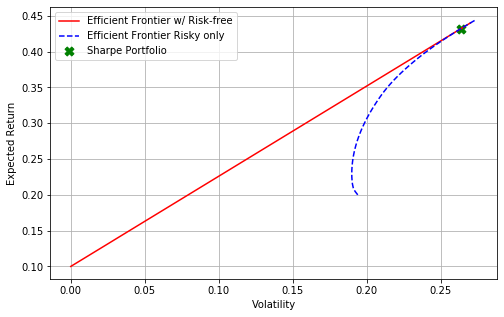
\includegraphics[width=0.7\textwidth]{figures/sharpe_ratio.png}
	\caption{Sharpe portfolio (green cross) compared to the efficient frontier with a risk-free asset (red) and with risky asset only (blue).}
	\label{fig:sharpe_ratio}
\end{figure}

So the optimization using the Sharpe ratio gives us a portfolio that is
on the minimum volatility efficient frontier, and gives the maximum
return relative to putting all our money in the risk-free asset.

Usually, any Sharpe ratio greater than 1.0 is considered acceptable to good by investors. A ratio higher than 2.0 is rated as very good. A ratio of 3.0 or higher is considered excellent. A ratio under 1.0 is sub-optimal.

\section{Capital Asset Pricing Model}
The Capital Asset Pricing Model (CAPM) describes the relationship between expected return of assets and systematic risk of the market.

CAPM states that the expected return of an asset is equal to the risk-free return plus a risk premium. The assumption of CAPM is that investors are rational and want to maximize return and reduce risk as much as possible so its goal is to calculate which return an investor can expect to make for a given risk premium over the risk-free rate.

Mathematically, we can summarize CAPM with the following formula
\begin{equation}
r_i = r_f + \beta_i(r_m-r_f)
\label{eq:capm}
\end{equation}
where:
\begin{itemize}
	\item $r_i$ is the expected return of the $i^{th}$ security;
	\item $r_f$ is the risk-free rate with zero standard deviation (an example of a risk-free asset includes Treasury Bills as they are backed by the U.S. government);
	\item $r_m - r_f$ is the risk premium ($r_m$ denotes the market return including all securities in the market, it can be represented with an index like S\&P 500);
	\item $\beta_i$ is a measure of $i^{th}$ asset volatility in relation to the overall market. 
	$\beta$ is used in the CAPM to describe the relationship between systematic risk, or market risk, and its expected return.
\end{itemize}
	
Therefore the key point in CAPM is the determination of $\beta$. This can be achieved with the measurement of the slope of the \emph{regression line}, of the market vs individual stock return distribution.

Given two sets of measurements $X$ and $y$ the linear regression determines the parameter $\alpha$ and $\beta$ such that

\[y=\beta X + \alpha\]
by minimizing the sum of the squared differences between the predicted and true $y$ values.
Figure~\ref{fig:linear_regression} shows an example of regression. 
In our case the regressed line estimates the stock returns given the global market returns and in particular 

\[\beta \approx \cfrac{\textrm{cov}(X,y)}{\textrm {var}(X)}\]
so provides insights about how \emph{volatile}, or how risky, a stock is relative to the rest of the market.
In CAPM $\beta$ calculation is used to help investors understand whether a stock moves in the same direction as the rest of the market but for it to provide any useful insight, the market that is used as a benchmark should be related to the stock.

If $\beta$ of an individual stock = 1.0, this means its price is perfectly correlated with the market, if $\beta < 1.0$, which is referred to as "defensive", this indicates the security is theoretically less volatile than the market (provides lower returns, so it is less risky), while if $\beta > 1.0$, or "aggressive", this indicates the assets price is more volatile than the market.

Those who use CAPM pick individual stocks or portfolios, and compare them to different indexes. The point is to find stocks that have high $\beta$, and portfolios that have high $\alpha$. High $\beta$ values mean that the stock fares better than index, so those stocks have a chance at beating the market. $\alpha$ values above zero mean that your portfolio gives positive return no matter what the market does.

\begin{figure}[htb]
	\centering
	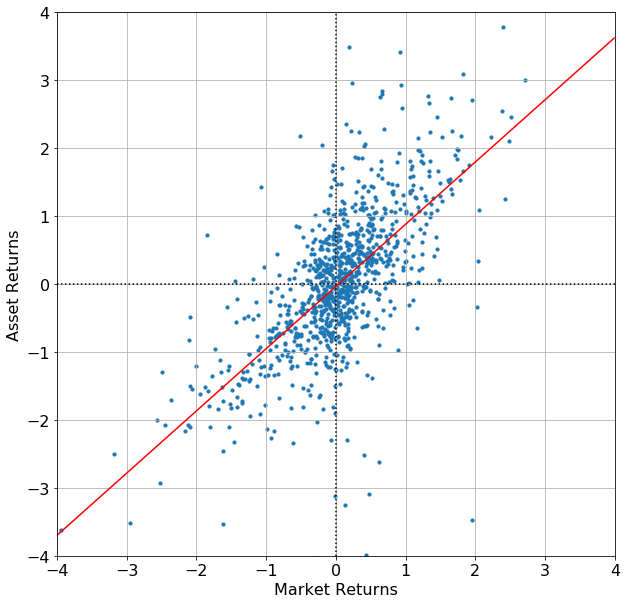
\includegraphics[width=0.7\textwidth]{figures/linear_regression}
	\caption{Example of linear regression for the determination of $\beta$.}
	\label{fig:linear_regression}
\end{figure}

In order to see an example of CAPM application we use \href{https://drive.google.com/file/d/1G4U8foyhq9agGPs8cg83-aY4qU8K3jJI/view?usp=sharing}{capm.csv} file which contains the historical series of S\&P500 and of some stocks.
As usual with \texttt{pandas} we can inspect the file and compute some useful quantities like daily and annualized expected returns.

\begin{tcolorbox}[breakable, size=fbox, boxrule=1pt, pad at break*=1mm,colback=cellbackground, colframe=cellborder]
\begin{Verbatim}[commandchars=\\\{\}]
\PY{k+kn}{import} \PY{n+nn}{pandas} \PY{k}{as} \PY{n+nn}{pd}
		
\PY{n}{capm} \PY{o}{=} \PY{n}{pd}\PY{o}{.}\PY{n}{read\PYZus{}csv}\PY{p}{(}\PY{l+s+s2}{\PYZdq{}}\PY{l+s+s2}{capm.csv}\PY{l+s+s2}{\PYZdq{}}\PY{p}{,} \PY{n}{index\PYZus{}col}\PY{o}{=}\PY{l+s+s1}{\PYZsq{}}\PY{l+s+s1}{date}\PY{l+s+s1}{\PYZsq{}}\PY{p}{)}
\PY{n+nb}{print} \PY{p}{(}\PY{n}{capm}\PY{o}{.}\PY{n}{head}\PY{p}{(}\PY{p}{)}\PY{p}{)}
\PY{n}{daily\PYZus{}returns} \PY{o}{=} \PY{n}{capm}\PY{o}{.}\PY{n}{pct\PYZus{}change}\PY{p}{(}\PY{p}{)}\PY{o}{*}\PY{l+m+mi}{100}

                 AAPL     AMZN          BA    GOOG         IBM        MGM 
date
27/03/2014  71.865678  338.470  111.078480  558.46  167.346339  24.629343
28/03/2014  71.785450  338.290  112.205402  559.99  167.892905  24.609560
31/03/2014  71.769404  336.365  113.133986  556.97  169.691285  25.578908
01/04/2014  72.425937  342.990  115.586169  567.16  171.463219  26.241625
02/04/2014  72.546280  341.960  115.676323  567.00  170.625738  26.409777

                    T    TSLA        SP500
date
27/03/2014  28.801410  207.32  1849.040039
28/03/2014  28.892032  212.37  1857.619995
31/03/2014  28.892032  208.45  1872.339966
01/04/2014  28.908509  216.97  1885.520020
02/04/2014  29.139184  230.29  1890.900024
\end{Verbatim}
\end{tcolorbox}

\subsubsection{Calculate $\beta$ and CAPM for each Stock}
To recap $\beta$ is the slope of the regression line of the market return vs stock return plot (and $\alpha$ is the intercept of this line with the $y$ axis).

These quantities can be calculated with \texttt{numpy.polyfit} passing as inputs the market and stock return lists. 
The resulting fits for the stocks in our sample are shown in Fig.~\ref{fig:capm_fit}.

With the daily returns and $\beta$ of each stock, we can apply the capital asset pricing model. First, we can calculate the average daily return of the market and annualize this return by multiplying it by the number of trading days in a year.
Assuming a risk-free rate of 1\%, we can then calculate CAPM using Eq.~\ref{eq:capm}.

\begin{tcolorbox}[breakable, size=fbox, boxrule=1pt, pad at break*=1mm,colback=cellbackground, colframe=cellborder]
\begin{Verbatim}[commandchars=\\\{\}]
\PY{n}{rm} \PY{o}{=} \PY{n}{np}\PY{o}{.}\PY{n}{mean}\PY{p}{(}\PY{n}{daily\PYZus{}returns}\PY{o}{.}\PY{n}{iloc}\PY{p}{[}\PY{l+m+mi}{1}\PY{p}{:}\PY{p}{]}\PY{p}{[}\PY{l+s+s1}{\PYZsq{}}\PY{l+s+s1}{SP500}\PY{l+s+s1}{\PYZsq{}}\PY{p}{]}\PY{p}{)}\PY{o}{*}\PY{l+m+mi}{252}
\PY{n}{rf} \PY{o}{=} \PY{l+m+mf}{0.01} 
	
\PY{n}{betas} \PY{o}{=} \PY{p}{\PYZob{}}\PY{p}{\PYZcb{}}
\PY{n}{alphas} \PY{o}{=} \PY{p}{\PYZob{}}\PY{p}{\PYZcb{}}
\PY{n}{ERs} \PY{o}{=} \PY{p}{\PYZob{}}\PY{p}{\PYZcb{}}
\PY{k}{for} \PY{n}{i}\PY{p}{,} \PY{n}{k} \PY{o+ow}{in} \PY{n+nb}{enumerate}\PY{p}{(}\PY{n}{df}\PY{o}{.}\PY{n}{columns}\PY{p}{)}\PY{p}{:}
    \PY{k}{if} \PY{n}{k} \PY{o}{==} \PY{l+s+s2}{\PYZdq{}}\PY{l+s+s2}{SP500}\PY{l+s+s2}{\PYZdq{}}\PY{p}{:}
        \PY{k}{continue}
    \PY{n}{betas}\PY{p}{[}\PY{n}{k}\PY{p}{]}\PY{p}{,} \PY{n}{alphas}\PY{p}{[}\PY{n}{k}\PY{p}{]} \PY{o}{=} \PY{n}{np}\PY{o}{.}\PY{n}{polyfit}\PY{p}{(}\PY{n}{daily\PYZus{}returns}\PY{p}{[}\PY{l+s+s1}{\PYZsq{}}\PY{l+s+s1}{SP500}\PY{l+s+s1}{\PYZsq{}}\PY{p}{]}\PY{p}{[}\PY{l+m+mi}{1}\PY{p}{:}\PY{p}{]}\PY{p}{,} 
    \PY{n}{daily\PYZus{}returns}\PY{p}{[}\PY{n}{k}\PY{p}{]}\PY{p}{[}\PY{l+m+mi}{1}\PY{p}{:}\PY{p}{]}\PY{p}{,} \PY{l+m+mi}{1}\PY{p}{)}
    \PY{n}{ERs}\PY{p}{[}\PY{n}{k}\PY{p}{]} \PY{o}{=} \PY{n}{rf} \PY{o}{+} \PY{p}{(}\PY{n}{betas}\PY{p}{[}\PY{n}{k}\PY{p}{]} \PY{o}{*} \PY{p}{(}\PY{n}{rm}\PY{o}{\PYZhy{}}\PY{n}{rf}\PY{p}{)}\PY{p}{)} 

\PY{k}{for} \PY{n}{k}\PY{p}{,} \PY{n}{v} \PY{o+ow}{in} \PY{n}{ERs}\PY{o}{.}\PY{n}{items}\PY{p}{(}\PY{p}{)}\PY{p}{:} 
\PY{n+nb}{print} \PY{p}{(}\PY{l+s+s2}{\PYZdq{}}\PY{l+s+si}{\PYZob{}:4\PYZcb{}}\PY{l+s+s2}{: }\PY{l+s+si}{\PYZob{}:4.1f\PYZcb{}}\PY{l+s+s2}{\PYZpc{}}\PY{l+s+s2}{\PYZdq{}}\PY{o}{.}\PY{n}{format}\PY{p}{(}\PY{n}{k}\PY{p}{,} \PY{n}{v}\PY{p}{)}\PY{p}{)}

AAPL: 10.3\%
AMZN: 10.8\%
BA  : 10.3\%
GOOG: 10.7\%
IBM :  8.7\%
MGM : 13.8\%
T   :  5.9\%
TSLA: 11.9\%
\end{Verbatim}
\end{tcolorbox}

\begin{figure}[htb]
	\centering
	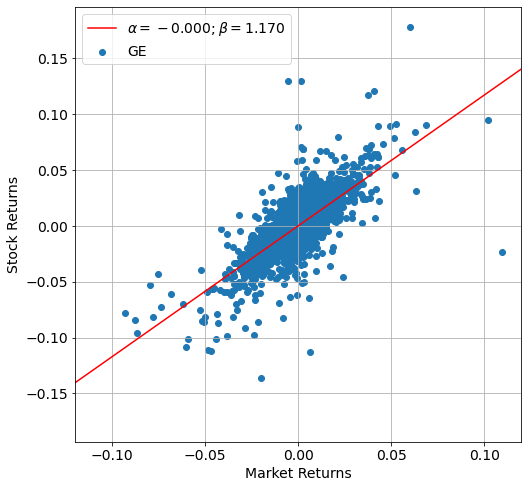
\includegraphics[width=.8\textwidth]{figures/capm_fit.png}
	\caption{Linear regression of market return vs stock return for a set of selected stocks. The fit results are also shown in red and the regression parameters are indicated in the legend.}
	\label{fig:capm_fit}
\end{figure}

Now that we have the $\beta$s of each individual stock we can calculate the CAPM for a portfolio made of the same stocks (we assume equal weights for simplicity).
It is enough indeed to perform a weighted sum of of the expected return according to the model of each stock.

\begin{tcolorbox}[breakable, size=fbox, boxrule=1pt, pad at break*=1mm,colback=cellbackground, colframe=cellborder]
\begin{Verbatim}[commandchars=\\\{\}]
\PY{n+nb}{print} \PY{p}{(}\PY{l+s+s2}{\PYZdq{}}\PY{l+s+si}{\PYZob{}:.1f\PYZcb{}}\PY{l+s+s2}{\PYZpc{}}\PY{l+s+s2}{\PYZdq{}}\PY{o}{.}\PY{n}{format}\PY{p}{(}\PY{n+nb}{sum}\PY{p}{(}\PY{n}{ERs}\PY{o}{.}\PY{n}{values}\PY{p}{(}\PY{p}{)}\PY{p}{)}\PY{o}{*}\PY{l+m+mi}{1}\PY{o}{/}\PY{n+nb}{len}\PY{p}{(}\PY{n}{ERs}\PY{p}{)}\PY{p}{)}\PY{p}{)}

10.3\%
\end{Verbatim}
\end{tcolorbox}

The expected return of the portfolio is roughly 10\% and this is what an investor should expect according to CAPM.

As we have seen the whole model is about plotting a line in a scatter plot, it’s not a very complex model. Assumptions under the model are even more simplistic. For example:
\begin{itemize}
\tightlist
\item expect that all investors are rational and they avoid risk;
\item everyone have full information about the market;
\item everyone have similar investment horizons and expectations about future movements;
\item stocks are all correctly priced.
\end{itemize}

Moreover, this is a model from the 1950s. Market dynamics were different back then. And of course, this is a retrospective model. We cannot know how future stock prices move and how the market behaves.
Interesting extension of CAPM involves \emph{Bayesian regression} but it will not be discussed here.

\section{Risk Parity Portfolio}
\label{risk-parity-portfolio}

An alternative approach to Markowitz theory is given by the
\emph{risk parity}. A risk parity portfolio is an investment allocation
strategy which focuses on the allocation of risk, rather than on the
allocation of capital. 
A risk parity (equal risk) portfolio is characterised by having equal risk contributions to the total risk from each individual asset. 

Risk parity allocation is also referred to as equally-weighted risk
contributions portfolio method. Equally-weighted risk contributions is
not about \emph{having the same volatility}, it is about having each
asset contributing in the same way to the portfolio overall volatility.
For this we will have to define the contribution of each asset to the
portfolio risk. 

This allocation strategy has gained popularity in the
last decades since it is believed to provide better risk adjusted return
than capital based allocation strategies.

Let's go over a very basic example to better illustrate how to construct
a simple risk parity (equal risk) portfolio. Later we will see how
to extend this technique to a risk budgeting portfolio (targeted risk
allocation).

Consider a portfolio of \(N\) assets: \(x_{1}, \ldots, x_N\) where as
usual the weight of the $i^{th}$ asset is denoted by \(w_{i}\). The
\(w_{i}\) form the allocation vector \(\mathbf{w}\). Let us further
denote the covariance matrix of the assets as \(\Sigma\). The volatility
of the portfolio is then defined as:

\[ \sigma_p={\sqrt {\mathbf{w^T}\Sigma \mathbf{w}}} = \sum_{i=1}^{N}\sigma _{i}\qquad\textrm{with}~\sigma _{i} = w_{i}\cdot \cfrac{\partial\sigma_p}{\partial w_{i}}={\cfrac {w_{i}(\Sigma \mathbf{w})_{i}}{\sqrt {\mathbf{w^T}\Sigma \mathbf{w}}}}\]
so that \(\sigma _{i}\) can be interpreted as the contribution of the $i^{th}$ asset to the overall risk of the portfolio.

\begin{tcolorbox}[breakable, size=fbox, boxrule=1pt, pad at break*=1mm,colback=cream, colframe=cellborder]
This paragraph can be skipped if you are not interested in the derivation of the $\sigma_i$.

Expressing explicitly in matrix form the standard deviation of the portfolio we get
\[
\begin{split}
	\sigma_p={\sqrt {\mathbf{w^T}\Sigma \mathbf{w}}} & =
	\sqrt{
		\begin{bmatrix}
			w_{1} \\
			w_{2}
		\end{bmatrix}
		\begin{bmatrix}
			\sigma_{11} & \sigma_{21} \\
			\sigma_{12} & \sigma_{22} 
		\end{bmatrix}
		\begin{bmatrix}
			w_{1} & w_{2} \\
		\end{bmatrix}
	}\\
	&=
	\sqrt{
		\begin{bmatrix}
			w_{1} \\
			w_{2}
		\end{bmatrix}
		\begin{bmatrix}
			w_{1}\sigma_{11} + w_{2}\sigma_{21} & w_{1}\sigma_{12} + w_{2}\sigma_{22} \\
		\end{bmatrix}
	} \\
	&= \sqrt{
		w_{1}w_{1}\sigma_{11} + w_{2}w_{1}\sigma_{21} + w_{1}w_{2}\sigma_{12} + w_{2}w_{2}\sigma_{22} }
\end{split}
\]
Now performing for example the derivative with respect to $w_1$ we obtain
\[\cfrac{\partial\sigma_p}{\partial w_1} = \cfrac{1}{2}\cdot\cfrac{2\cdot w_1\sigma_{11} + 2\cdot w_{2}\sigma_{21}}{\sigma_p} = \cfrac{w_1\sigma_{11} + w_{2}\sigma_{21}}{\sigma_p} = \cfrac{(\Sigma \mathbf{w})_{1}}{\sigma_p}\]

Summing up $\sum w_i\cdot\cfrac{\partial\sigma_p}{\partial w_i}$ we get back $\sigma_p$
\end{tcolorbox}

Equal risk contribution then means \(\sigma _{i} =\sigma _{j}\) for all
\(i,j\) or equivalently \(\sigma _{i}=\sigma_p/N\). So

\[\sigma _{i} = \cfrac{\sigma_p}{N}={\cfrac {w_{i}(\Sigma \mathbf{w})_{i}}{\sqrt {\mathbf{w^T}\Sigma \mathbf{w}}}}\implies w_{i} = \frac {\sigma_p^{2}}{(\Sigma \mathbf{w})_{i}N}\]
Since we want the previous expression to be true for each $i$, the solution for the weights can be found by solving the minimisation problem

\[ \underset{\mathbf{w}}{\min } \sum _{i=1}^{N}\left[w_{i}-{\frac {\sigma_p^{2}}{(\Sigma \mathbf{w})_{i}N}}\right]^{2} \]

Going back to our data sample let's find out the weights to give us a
risk parity portfolio.

\begin{tcolorbox}[breakable, size=fbox, boxrule=1pt, pad at break*=1mm,colback=cellbackground, colframe=cellborder]
\begin{Verbatim}[commandchars=\\\{\}]
\PY{n}{num\PYZus{}assets} \PY{o}{=} \PY{l+m+mi}{5}
\PY{k}{def} \PY{n+nf}{risk\PYZus{}parity}\PY{p}{(}\PY{n}{w}\PY{p}{,} \PY{n}{cov}\PY{p}{)}\PY{p}{:}
    \PY{n}{variance} \PY{o}{=} \PY{n}{w}\PY{o}{.}\PY{n}{T}\PY{o}{.}\PY{n}{dot}\PY{p}{(}\PY{n}{cov}\PY{o}{.}\PY{n}{dot}\PY{p}{(}\PY{n}{w}\PY{p}{)}\PY{p}{)} 
    \PY{n+nb}{sum} \PY{o}{=} \PY{l+m+mi}{0}
    \PY{n}{N} \PY{o}{=} \PY{n+nb}{len}\PY{p}{(}\PY{n}{w}\PY{p}{)}
    \PY{k}{for} \PY{n}{i} \PY{o+ow}{in} \PY{n+nb}{range}\PY{p}{(}\PY{n}{N}\PY{p}{)}\PY{p}{:}
        \PY{n+nb}{sum} \PY{o}{+}\PY{o}{=} \PY{p}{(}\PY{n}{w}\PY{p}{[}\PY{n}{i}\PY{p}{]} \PY{o}{\PYZhy{}} \PY{p}{(}\PY{n}{variance}\PY{o}{/}\PY{p}{(}\PY{n}{N}\PY{o}{*}\PY{n}{cov}\PY{o}{.}\PY{n}{dot}\PY{p}{(}\PY{n}{w}\PY{p}{)}\PY{p}{[}\PY{n}{i}\PY{p}{]}\PY{p}{)}\PY{p}{)}\PY{p}{)}\PY{o}{*}\PY{o}{*}\PY{l+m+mi}{2} 
    \PY{k}{return} \PY{n+nb}{sum}
		
\PY{n}{args} \PY{o}{=} \PY{p}{(}\PY{n}{covariance}\PY{p}{,}\PY{p}{)}
\PY{n}{constraints} \PY{o}{=} \PY{p}{(}\PY{p}{\PYZob{}}\PY{l+s+s1}{\PYZsq{}}\PY{l+s+s1}{type}\PY{l+s+s1}{\PYZsq{}}\PY{p}{:} \PY{l+s+s1}{\PYZsq{}}\PY{l+s+s1}{eq}\PY{l+s+s1}{\PYZsq{}}\PY{p}{,} \PY{l+s+s1}{\PYZsq{}}\PY{l+s+s1}{fun}\PY{l+s+s1}{\PYZsq{}}\PY{p}{:} \PY{n}{sum\PYZus{}weights}\PY{p}{\PYZcb{}}\PY{p}{)} 
\PY{n}{bounds} \PY{o}{=} \PY{n+nb}{tuple}\PY{p}{(}\PY{p}{(}\PY{l+m+mi}{0}\PY{p}{,} \PY{l+m+mi}{1}\PY{p}{)} \PY{k}{for} \PY{n}{asset} \PY{o+ow}{in} \PY{n+nb}{range}\PY{p}{(}\PY{n}{num\PYZus{}assets}\PY{p}{)}\PY{p}{)}
\PY{n}{weights} \PY{o}{=} \PY{p}{[}\PY{l+m+mf}{1.}\PY{o}{/}\PY{n}{num\PYZus{}assets} \PY{k}{for} \PY{n}{\PYZus{}} \PY{o+ow}{in} \PY{n+nb}{range}\PY{p}{(}\PY{n}{num\PYZus{}assets}\PY{p}{)}\PY{p}{]}
\PY{n}{opts} \PY{o}{=} \PY{n}{minimize}\PY{p}{(}\PY{n}{risk\PYZus{}parity}\PY{p}{,} \PY{n}{weights}\PY{p}{,} \PY{n}{args}\PY{o}{=}\PY{p}{(}\PY{n}{covariance}\PY{p}{,}\PY{p}{)}\PY{p}{,}
                \PY{n}{bounds}\PY{o}{=}\PY{n}{bounds}\PY{p}{,} \PY{n}{constraints}\PY{o}{=}\PY{n}{constraints}\PY{p}{)}
\PY{n+nb}{print} \PY{p}{(}\PY{n}{opts}\PY{p}{)}

    fun: 2.2543755363349716e-07
    jac: array([-7.06474804e-04,  1.97343062e-04, -4.26326934e-05,
                -8.04037852e-06,  1.11882164e-03])
message: 'Optimization terminated successfully.'
   nfev: 38
    nit: 5 
   njev: 5
 status: 0
success: True
      x: array([0.25895309, 0.18118756, 0.19670379, 0.22208923, 
                0.14106633])

\PY{n}{sigma\PYZus{}i} \PY{o}{=} \PY{p}{[}\PY{p}{]}
\PY{k}{for} \PY{n}{i} \PY{o+ow}{in} \PY{n+nb}{range}\PY{p}{(}\PY{n}{num\PYZus{}assets}\PY{p}{)}\PY{p}{:}
    \PY{n}{std} \PY{o}{=} \PY{n}{np}\PY{o}{.}\PY{n}{sqrt}\PY{p}{(}\PY{n}{opts}\PY{o}{.}\PY{n}{x}\PY{o}{.}\PY{n}{T}\PY{o}{.}\PY{n}{dot}\PY{p}{(}\PY{n}{covariance}\PY{o}{.}\PY{n}{dot}\PY{p}{(}\PY{n}{opts}\PY{o}{.}\PY{n}{x}\PY{p}{)}\PY{p}{)}\PY{p}{)} 
    \PY{n}{a} \PY{o}{=} \PY{n}{opts}\PY{o}{.}\PY{n}{x}\PY{p}{[}\PY{n}{i}\PY{p}{]}\PY{o}{*}\PY{n}{covariance}\PY{o}{.}\PY{n}{dot}\PY{p}{(}\PY{n}{opts}\PY{o}{.}\PY{n}{x}\PY{p}{)}\PY{p}{[}\PY{n}{i}\PY{p}{]} 
    \PY{n}{sigma\PYZus{}i}\PY{o}{.}\PY{n}{append}\PY{p}{(}\PY{n}{a}\PY{o}{/}\PY{n}{std}\PY{p}{)}
		
\PY{k}{for} \PY{n}{i} \PY{o+ow}{in} \PY{n+nb}{range}\PY{p}{(}\PY{n}{num\PYZus{}assets}\PY{p}{)}\PY{p}{:}
    \PY{n+nb}{print} \PY{p}{(}\PY{l+s+s2}{\PYZdq{}}\PY{l+s+s2}{Risk contribution for asset }\PY{l+s+si}{\PYZob{}\PYZcb{}}\PY{l+s+s2}{: }\PY{l+s+si}{\PYZob{}:.3f\PYZcb{}}\PY{l+s+s2}{\PYZpc{}}\PY{l+s+s2}{\PYZdq{}}
           \PY{o}{.}\PY{n}{format}\PY{p}{(}\PY{n}{i}\PY{p}{,} \PY{n}{sigma\PYZus{}i}\PY{p}{[}\PY{n}{i}\PY{p}{]}\PY{o}{/}\PY{n+nb}{sum}\PY{p}{(}\PY{n}{sigma\PYZus{}i}\PY{p}{)}\PY{o}{*}\PY{l+m+mi}{100}\PY{p}{)}\PY{p}{)}

Risk contribution for asset 0: 19.974\%
Risk contribution for asset 1: 19.999\%
Risk contribution for asset 2: 19.990\%
Risk contribution for asset 3: 19.993\%
Risk contribution for asset 4: 20.044\%
\end{Verbatim}
\end{tcolorbox}

%Figure~\ref{fig:risk_parity} shows the fraction of risk allocated to each asset and the corresponding weight within the portfolio.

\subsection{Risk Budget Allocation}
\label{risk-budget-allocation}

The same technique can be used if we would like to calculate a portfolio
with risk budget allocation. In this case we want to associate to each asset a particular level of risk. If we consider the previous equation

\[ \sigma _{i}=\cfrac{\sigma_p}{N} \]
where we set the risk contribution fraction to every asset to \(1/N\);
now we can simply replace \(1/N\) with the desired fraction of risk (\(f_i\)) for each asset

\[ \sigma _{i}=f_i \cdot \sigma_p \]
so that the relation to minimise becomes

\[ \underset{\mathbf{w}}{\min} \sum _{i=1}^{N}\left[w_{i}-{\frac {f_i \cdot \sigma_p^{2}}{(\Sigma \mathbf{w})_{i}}}\right]^{2} \]

Translating it into \texttt{python} we get:

\begin{tcolorbox}[breakable, size=fbox, boxrule=1pt, pad at break*=1mm,colback=cellbackground, colframe=cellborder]
\begin{Verbatim}[commandchars=\\\{\}]
\PY{k}{def} \PY{n+nf}{risk\PYZus{}budget}\PY{p}{(}\PY{n}{w}\PY{p}{,} \PY{n}{target\PYZus{}risk}\PY{p}{,} \PY{n}{cov}\PY{p}{)}\PY{p}{:}
    \PY{n}{variance} \PY{o}{=} \PY{n}{w}\PY{o}{.}\PY{n}{T}\PY{o}{.}\PY{n}{dot}\PY{p}{(}\PY{n}{cov}\PY{o}{.}\PY{n}{dot}\PY{p}{(}\PY{n}{w}\PY{p}{)}\PY{p}{)} 
    \PY{n+nb}{sum} \PY{o}{=} \PY{l+m+mi}{0}
    \PY{n}{N} \PY{o}{=} \PY{n+nb}{len}\PY{p}{(}\PY{n}{w}\PY{p}{)}
    \PY{k}{for} \PY{n}{i} \PY{o+ow}{in} \PY{n+nb}{range}\PY{p}{(}\PY{n}{N}\PY{p}{)}\PY{p}{:}
        \PY{n+nb}{sum} \PY{o}{+}\PY{o}{=} \PY{p}{(}\PY{n}{w}\PY{p}{[}\PY{n}{i}\PY{p}{]} \PY{o}{\PYZhy{}} \PY{p}{(}\PY{n}{target\PYZus{}risk}\PY{p}{[}\PY{n}{i}\PY{p}{]}\PY{o}{*}\PY{n}{variance}\PY{p}{)}\PY{o}{/}\PY{p}{(}\PY{n}{cov}\PY{o}{.}\PY{n}{dot}\PY{p}{(}\PY{n}{w}\PY{p}{)}\PY{p}{[}\PY{n}{i}\PY{p}{]}\PY{p}{)}\PY{p}{)}\PY{o}{*}\PY{o}{*}\PY{l+m+mi}{2} 
    \PY{k}{return} \PY{n+nb}{sum}
		
\PY{n}{f\PYZus{}i} \PY{o}{=} \PY{p}{[}\PY{l+m+mf}{0.3}\PY{p}{,} \PY{l+m+mf}{0.2}\PY{p}{,} \PY{l+m+mf}{0.2}\PY{p}{,} \PY{l+m+mf}{0.15}\PY{p}{,} \PY{l+m+mf}{0.15}\PY{p}{]} 
\PY{n}{args} \PY{o}{=} \PY{p}{(}\PY{n}{f\PYZus{}i}\PY{p}{,} \PY{n}{covariance}\PY{p}{)}
\PY{n}{constraints} \PY{o}{=} \PY{p}{(}\PY{p}{\PYZob{}}\PY{l+s+s1}{\PYZsq{}}\PY{l+s+s1}{type}\PY{l+s+s1}{\PYZsq{}}\PY{p}{:} \PY{l+s+s1}{\PYZsq{}}\PY{l+s+s1}{eq}\PY{l+s+s1}{\PYZsq{}}\PY{p}{,} \PY{l+s+s1}{\PYZsq{}}\PY{l+s+s1}{fun}\PY{l+s+s1}{\PYZsq{}}\PY{p}{:} \PY{n}{sum\PYZus{}weights}\PY{p}{\PYZcb{}}\PY{p}{)}          
\PY{n}{bounds} \PY{o}{=} \PY{n+nb}{tuple}\PY{p}{(}\PY{p}{(}\PY{l+m+mi}{0}\PY{p}{,} \PY{l+m+mi}{1}\PY{p}{)} \PY{k}{for} \PY{n}{asset} \PY{o+ow}{in} \PY{n+nb}{range}\PY{p}{(}\PY{n}{num\PYZus{}assets}\PY{p}{)}\PY{p}{)}
\PY{n}{weights} \PY{o}{=} \PY{p}{[}\PY{l+m+mf}{1.}\PY{o}{/}\PY{n}{num\PYZus{}assets} \PY{k}{for} \PY{n}{\PYZus{}} \PY{o+ow}{in} \PY{n+nb}{range}\PY{p}{(}\PY{n}{num\PYZus{}assets}\PY{p}{)}\PY{p}{]}
\PY{n}{opts} \PY{o}{=} \PY{n}{minimize}\PY{p}{(}\PY{n}{risk\PYZus{}budget}\PY{p}{,} \PY{n}{weights}\PY{p}{,} \PY{n}{args}\PY{o}{=}\PY{p}{(}\PY{n}{f\PYZus{}i}\PY{p}{,} \PY{n}{covariance}\PY{p}{)}\PY{p}{,} 
                \PY{n}{bounds}\PY{o}{=}\PY{n}{bounds}\PY{p}{,} \PY{n}{constraints}\PY{o}{=}\PY{n}{constraints}\PY{p}{)}
\PY{n+nb}{print} \PY{p}{(}\PY{n}{opts}\PY{p}{)}
		
    fun: 4.798712878867406e-08
    jac: array([-3.11920407e-04,  3.24431247e-04,  
                 9.84173665e-05, -9.10631775e-05,  4.14667119e-04])
message: 'Optimization terminated successfully.'
   nfev: 45
    nit: 6
   njev: 6
 status: 0
success: True
      x: array([0.34604471, 0.17973628, 0.19407208, 0.16911722, 
                0.11102971])
		
\PY{n}{sigma\PYZus{}i} \PY{o}{=} \PY{p}{[}\PY{p}{]}
\PY{k}{for} \PY{n}{i} \PY{o+ow}{in} \PY{n+nb}{range}\PY{p}{(}\PY{n}{num\PYZus{}assets}\PY{p}{)}\PY{p}{:}
    \PY{n}{std} \PY{o}{=} \PY{n}{np}\PY{o}{.}\PY{n}{sqrt}\PY{p}{(}\PY{n}{opts}\PY{o}{.}\PY{n}{x}\PY{o}{.}\PY{n}{T}\PY{o}{.}\PY{n}{dot}\PY{p}{(}\PY{n}{covariance}\PY{o}{.}\PY{n}{dot}\PY{p}{(}\PY{n}{opts}\PY{o}{.}\PY{n}{x}\PY{p}{)}\PY{p}{)}\PY{p}{)} 
    \PY{n}{a} \PY{o}{=} \PY{n}{opts}\PY{o}{.}\PY{n}{x}\PY{p}{[}\PY{n}{i}\PY{p}{]}\PY{o}{*}\PY{n}{covariance}\PY{o}{.}\PY{n}{dot}\PY{p}{(}\PY{n}{opts}\PY{o}{.}\PY{n}{x}\PY{p}{)}\PY{p}{[}\PY{n}{i}\PY{p}{]} 
    \PY{n}{sigma\PYZus{}i}\PY{o}{.}\PY{n}{append}\PY{p}{(}\PY{n}{a}\PY{o}{/}\PY{n}{std}\PY{p}{)}
		
\PY{k}{for} \PY{n}{i} \PY{o+ow}{in} \PY{n+nb}{range}\PY{p}{(}\PY{n}{num\PYZus{}assets}\PY{p}{)}\PY{p}{:}
    \PY{n+nb}{print} \PY{p}{(}\PY{l+s+s2}{\PYZdq{}}\PY{l+s+s2}{Risk contribution for asset }\PY{l+s+si}{\PYZob{}\PYZcb{}}\PY{l+s+s2}{: }\PY{l+s+si}{\PYZob{}:.3f\PYZcb{}}\PY{l+s+s2}{\PYZpc{}}\PY{l+s+s2}{\PYZdq{}}
            \PY{o}{.}\PY{n}{format}\PY{p}{(}\PY{n}{i}\PY{p}{,} \PY{n}{sigma\PYZus{}i}\PY{p}{[}\PY{n}{i}\PY{p}{]}\PY{o}{/}\PY{n+nb}{sum}\PY{p}{(}\PY{n}{sigma\PYZus{}i}\PY{p}{)}\PY{o}{*}\PY{l+m+mi}{100}\PY{p}{)}\PY{p}{)}
		
Risk contribution for asset 0: 29.986\%
Risk contribution for asset 1: 20.009\%
Risk contribution for asset 2: 19.999\%
Risk contribution for asset 3: 14.992\%
Risk contribution for asset 4: 15.013\%
\end{Verbatim}
\end{tcolorbox}

%Figure~\ref{risk_allocation} shows the amount of risk associated to each asset and their weights within the portfolio. 
Indeed for each stock we have allocated the desired amount of risk.

\section{Maximum Diversification Portfolio}
\label{maximum-diversification-portfolio}

In addition to minimum variance, and risk parity/budgeting, maximum diversification is also another well known risk based asset allocation technique.

Diversification is a common topic in portfolio construction. Rather than serving as the sole, quantifiable objective, it is most often either pursued in tandem with another objective, such as return maximization, or pursued simply by including more asset classes or adding constraints based on intuition.

But it does not have to be this way and diversification can be pursued explicitly as the sole objective in portfolio construction.
In a 2008 paper, the diversification ratio $D$ of a portfolio has been defined as

\[
D=\cfrac{\mathbf{w^T}\boldsymbol{\sigma}}{\sqrt {\mathbf{w^T}\Sigma \mathbf{w}}} 
\]
where $\boldsymbol{\sigma}$ is the vector of volatilities and $\Sigma$ is the covariance matrix. The denominator represents the volatility of the portfolio and the numerator the weighted average volatility of the assets. More diversification within a portfolio decreases the denominator and leads to a higher diversification ratio.
Let's construct a portfolio that maximize this ratio.

\begin{tcolorbox}[breakable, size=fbox, boxrule=1pt, pad at break*=1mm,colback=cellbackground, colframe=cellborder]
\begin{Verbatim}[commandchars=\\\{\}]
\PY{k}{def} \PY{n+nf}{diversification\PYZus{}ratio}\PY{p}{(}\PY{n}{w}\PY{p}{)}\PY{p}{:}
    \PY{n}{w\PYZus{}vol} \PY{o}{=} \PY{n}{np}\PY{o}{.}\PY{n}{dot}\PY{p}{(}\PY{n}{np}\PY{o}{.}\PY{n}{sqrt}\PY{p}{(}\PY{n}{np}\PY{o}{.}\PY{n}{diag}\PY{p}{(}\PY{n}{covariance}\PY{p}{)}\PY{p}{)}\PY{p}{,} \PY{n}{w}\PY{o}{.}\PY{n}{T}\PY{p}{)}
    \PY{n}{port\PYZus{}vol} \PY{o}{=} \PY{n}{np}\PY{o}{.}\PY{n}{sqrt}\PY{p}{(}\PY{n}{np}\PY{o}{.}\PY{n}{dot}\PY{p}{(}\PY{n}{w}\PY{o}{.}\PY{n}{T}\PY{p}{,} \PY{n}{np}\PY{o}{.}\PY{n}{dot}\PY{p}{(}\PY{n}{covariance}\PY{p}{,} \PY{n}{w}\PY{p}{)}\PY{p}{)}\PY{p}{)}
    \PY{n}{diversification\PYZus{}ratio} \PY{o}{=} \PY{n}{w\PYZus{}vol}\PY{o}{/}\PY{n}{port\PYZus{}vol}
    \PY{k}{return} \PY{o}{\PYZhy{}}\PY{n}{diversification\PYZus{}ratio}
	
\PY{n}{bounds} \PY{o}{=} \PY{n+nb}{tuple}\PY{p}{(}\PY{p}{(}\PY{l+m+mi}{0}\PY{p}{,} \PY{l+m+mi}{1}\PY{p}{)} \PY{k}{for} \PY{n}{asset} \PY{o+ow}{in} \PY{n+nb}{range}\PY{p}{(}\PY{n}{num\PYZus{}assets}\PY{p}{)}\PY{p}{)}
\PY{n}{cons} \PY{o}{=} \PY{p}{(}\PY{p}{\PYZob{}}\PY{l+s+s1}{\PYZsq{}}\PY{l+s+s1}{type}\PY{l+s+s1}{\PYZsq{}}\PY{p}{:} \PY{l+s+s1}{\PYZsq{}}\PY{l+s+s1}{eq}\PY{l+s+s1}{\PYZsq{}}\PY{p}{,} \PY{l+s+s1}{\PYZsq{}}\PY{l+s+s1}{fun}\PY{l+s+s1}{\PYZsq{}}\PY{p}{:} \PY{n}{sum\PYZus{}weights}\PY{p}{\PYZcb{}}\PY{p}{,}\PY{p}{)}
\PY{c+c1}{\PYZsh{}cons = cons + (\PYZob{}\PYZsq{}type\PYZsq{}: \PYZsq{}ineq\PYZsq{}, \PYZsq{}fun\PYZsq{}:  long\PYZus{}only\PYZus{}constraint\PYZcb{},)}
\PY{n}{weights} \PY{o}{=} \PY{p}{[}\PY{l+m+mf}{1.}\PY{o}{/}\PY{n}{num\PYZus{}assets} \PY{k}{for} \PY{n}{\PYZus{}} \PY{o+ow}{in} \PY{n+nb}{range}\PY{p}{(}\PY{n}{num\PYZus{}assets}\PY{p}{)}\PY{p}{]}
	
\PY{n}{opts} \PY{o}{=} \PY{n}{minimize}\PY{p}{(}\PY{n}{diversification\PYZus{}ratio}\PY{p}{,} \PY{n}{weights}\PY{p}{,} \PY{n}{bounds}\PY{o}{=}\PY{n}{bounds}\PY{p}{,} 
                \PY{n}{constraints}\PY{o}{=}\PY{n}{cons}\PY{p}{)}
	
\PY{n+nb}{print} \PY{p}{(}\PY{n}{opts}\PY{p}{)}

    fun: -1.3603935531589488
    jac: array([-0.00038704,  0.00023621, -0.00032043,  0.00083792,  
                0.00020067])
message: 'Optimization terminated successfully.'
   nfev: 37
    nit: 5
   njev: 5
 status: 0
success: True
      x: array([0.3495816 , 0.17887765, 0.1566318 , 0.12398934, 
                0.19091962])

\PY{n}{ret} \PY{o}{=} \PY{n}{np}\PY{o}{.}\PY{n}{sum}\PY{p}{(}\PY{n}{returns}\PY{o}{*}\PY{n}{opts}\PY{o}{.}\PY{n}{x}\PY{p}{)}
\PY{n}{vol} \PY{o}{=} \PY{n}{np}\PY{o}{.}\PY{n}{sqrt}\PY{p}{(}\PY{n}{np}\PY{o}{.}\PY{n}{dot}\PY{p}{(}\PY{n}{opts}\PY{o}{.}\PY{n}{x}\PY{o}{.}\PY{n}{T}\PY{p}{,} \PY{n}{np}\PY{o}{.}\PY{n}{dot}\PY{p}{(}\PY{n}{covariance}\PY{p}{,} \PY{n}{opts}\PY{o}{.}\PY{n}{x}\PY{p}{)}\PY{p}{)}\PY{p}{)} 
\PY{n+nb}{print} \PY{p}{(}\PY{l+s+s2}{\PYZdq{}}\PY{l+s+s2}{Diversification: }\PY{l+s+s2}{\PYZdq{}}\PY{p}{,} \PY{o}{\PYZhy{}}\PY{n}{opts}\PY{o}{.}\PY{n}{fun}\PY{p}{)}

Diversification:  1.3603935531589488
\end{Verbatim}
\end{tcolorbox}

Figure~\ref{fig:max_div} shows how the maximum diversified portfolio compares to the efficient frontier.

\begin{figure}[htb]
	\centering
	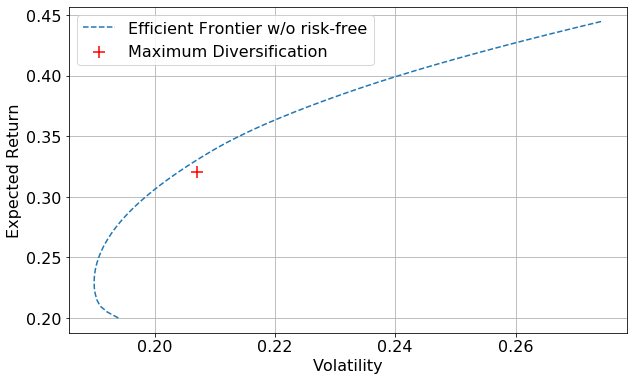
\includegraphics[width=0.7\textwidth]{figures/max_div.png}
	\caption{Portfolio constructed with the maximum diversification technique shown in the return/variance plane.}
	\label{fig:max_div}
\end{figure}
